\begin{figure}[!htbp]%
\centering
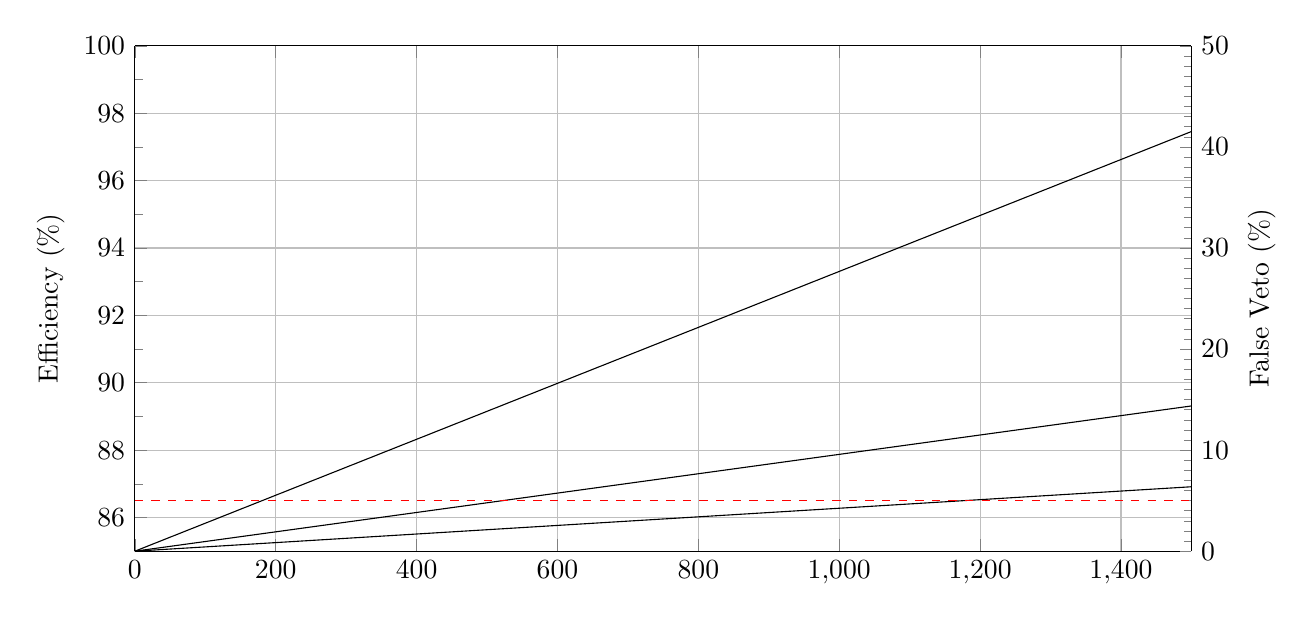
\begin{tikzpicture}
\centering
    \begin{axis}[
            ylabel=Efficiency (\%),
            width=15cm,
            height=8cm,
            grid=major,
            axis y line*=left,
            xmin=0, xmax=1500,
            ymin=85, ymax=100,
            minor y tick num=1,
            ]
    \end{axis}
    \begin{axis}[
            ylabel=False Veto (\%),
            yticklabel pos=right,
            axis y line*=right,
            axis x line=none,
            width=15cm,
            height=8cm,
            %grid=major,
            xmin=0, xmax=1500,
            ymin=0, ymax=50,
            minor y tick num=9,]
        \addplot[domain=0:1500,
            samples=3,
            ]
            {x * 42.5 * 100 / 1000000};
        \addplot[domain=0:1500,
            samples=3,
            ]
            {x * 95.8 * 100 / 1000000};        
        \addplot[domain=0:1500,
            samples=3,
            ]
            {x * 276.8 * 100 / 1000000};  
         \addplot[dashed, mark=none, red] coordinates {(0,5) (1500,5)};
    \end{axis}
            
\end{tikzpicture}
    \caption{Neutron tagging efficiency from AmLi at each height for the 200keV phe threshold}
    \label{fig:commissioning_amli_efficiency_with_bg_rate}
\end{figure}